\section{Further tests of information loss and decision value}\label{app:review_followthrough}
These analyses address different limits of the central comparison. They reuse stored answers and are exploratory; they add neither cases nor independent confirmation. Native288 uses its original four-model allocation. Native720 and Health256 use eight Gemma calls, eight Llama3.3-70B calls and the first four scheduled slots from each. Empty failed slots remain. Except for the explicitly labeled Monte Carlo reference distributions, intervals resample whole questions, average banks, and retain native task strata. A common 20,000-draw bootstrap (seed 20260921) supplies nominal intervals and the family adjustments specified below. The original primary intervals, obtained with their own frozen seeds and 50,000 draws, remain authoritative.

\subsection{Prespecified endpoints and generation failures}
The representation study froze native $C$ before new generation; MedEinst was a prespecified secondary transport with uncertain mappings. The 720-question study froze first-choice $\theta$ after development-only selection among ten homogeneous policies. Health froze $C_G$ before its generations. The later fifteen-policy search was specified after test outcomes were known, but selected its winner using development data only. K1/K5 generated fresh answers on 128 new questions under a separately frozen contract comparison; its unresolved primary missed the precision target. Depth, budget, partner, rank-transfer, information-bound, relabeling, screening and oracle results are saved-output analyses, not additional replications. The held-out predictor's recipe was frozen after generation began but before fresh accuracy analysis.

The original attempt audit reconciles 13,440 slots with 13,845 attempts, first-valid retention and at most one identical-payload retry. Every source/model cell passes the protocol's terminal-failure threshold of at most 5\% (Table~\ref{tab:failure_cells}). A failed first attempt followed by success is an attempted retry, not a terminal failed slot. Meeting this failure threshold does not resolve scoring or scientific transport uncertainty.

\begin{table}[ht]
\centering\small
\caption{Original representation study: scheduled slots, actual attempts including retries, terminal failures and percentage of scheduled slots failing. All eight source/model cells are below the prespecified 5\% failure limit.}
\label{tab:failure_cells}
\begin{tabular}{llrrrr}
\toprule
Source & Model & Slots & Attempts & Failures & \%\\
\midrule
medeinst & gemma & 3072 & 3104 & 5 & 0.16\\
medeinst & llama & 768 & 788 & 0 & 0.00\\
medeinst & ministral & 768 & 773 & 2 & 0.26\\
medeinst & qwen & 768 & 771 & 1 & 0.13\\
native & gemma & 4608 & 4863 & 85 & 1.84\\
native & llama & 1152 & 1218 & 43 & 3.73\\
native & ministral & 1152 & 1153 & 0 & 0.00\\
native & qwen & 1152 & 1175 & 12 & 1.04\\
\bottomrule
\end{tabular}
\end{table}

\subsection{Tie accounting and rule-eligible selection}
For each question, define $T=(F_{H,\mathrm{tie}}-F_{H,\mathrm{incl}})-(F_{M,\mathrm{tie}}-F_{M,\mathrm{incl}})$ and $U=(F_{M,\mathrm{tie}}-F_{H,\mathrm{tie}})-(F_{M,\mathrm{first}}-F_{H,\mathrm{first}})$. Then $C=T+U$ exactly before and after averaging. Six component endpoints (three cohorts, $T/U$) share a Bonferroni family. The unresolved remainders do not establish equivalence. Conditioning on observed masking is descriptive: the contribution from questions with at least one correct unanimous H first-choice bank masked by an inclusion tie is calculated using the full cohort denominator, not as a subgroup average.

\begin{table}[ht]
\centering\small
\caption{Paired decomposition in percentage points. T/U intervals adjust across six components. Masked and other contributions sum to C; their columns are point estimates using the full question denominator.}
\begin{tabular}{lrrrr}
\toprule
Cohort & T [adjusted 95\%] & U [adjusted 95\%] & Masked & Other\\
\midrule
Native288 & $7.62\ [2.04,13.32]$ & $2.10\ [-1.85,6.11]$ & 6.90 & 2.82\\
Native720 & $8.73\ [5.48,11.95]$ & $0.45\ [-1.86,2.81]$ & 6.42 & 2.76\\
Health256 & $5.98\ [1.25,10.52]$ & $0.16\ [-2.80,3.19]$ & 9.06 & -2.92\\
\bottomrule
\end{tabular}
\end{table}

First-choice eligibility means that gold appears at rank one in at least one selected list. All-rank availability means it appears anywhere. We calculate conditional success as pooled final accuracy divided by pooled eligibility, recomputing both terms in each bootstrap. For first-choice voting, the error decomposes as $1-F=(1-v_1)+(v_1-F)$: inaccessible gold plus failure despite rank-one access. The denominator is the full set of scheduled questions and banks, including failures. The archive additionally reports minimum-gold-rank frequencies (ranks one to five, or absent), all-rank conditional success, and paired intervals.

The exact counts make the conditioning explicit. Native720 has 1,440 question--bank records: H/M have gold at any rank in 1,291/1,327 records and at rank one somewhere in 671/709. Their expected correct totals are $6085/12$ and $2269/6$, yielding $100(6085/12)/671=75.57\%$ and $100(2269/6)/709=53.34\%$ conditional success. Health has 512 records: all-rank counts 493/501, rank-one counts 380/411, and expected correct totals $1057/3$ and $693/2$, yielding 92.72/84.31\%. These fractional totals average uniform voting ties; they are not counts of independently observed successes. Resampling keeps both banks together within each question. Comparing conditional rates on different eligible sets is descriptive, not a matched intervention on selector ability.

\begin{table}[ht]
\centering\small
\caption{Eligibility and selection (percent). F/v1 uses pooled values; it is not an average of question-level ratios.}
\begin{tabular}{llrrrrr}
\toprule
Cohort & Policy & Rank-one v1 & All-rank v & F/v1 & Inaccessible & Eligible error\\
\midrule
Native288 & H & 43.75 & 86.28 & 68.25 & 56.25 & 13.89\\
Native288 & M & 50.17 & 89.58 & 37.69 & 49.83 & 31.26\\
Native720 & H & 46.60 & 89.65 & 75.57 & 53.40 & 11.38\\
Native720 & M & 49.24 & 92.15 & 53.34 & 50.76 & 22.97\\
Health256 & H & 74.22 & 96.29 & 92.72 & 25.78 & 5.40\\
Health256 & M & 80.27 & 97.85 & 84.31 & 19.73 & 12.60\\
\bottomrule
\end{tabular}
\end{table}

\begin{table}[ht]
\centering\small
\caption{Eight-call first-choice minus a uniformly selected scheduled single slot, using the same five-answer contract. Intervals adjust over four contrasts; neither interval type is evidence of equivalence.}
\begin{tabular}{llrr}
\toprule
Cohort & Policy & Gain [95\%] & Gain [adjusted 95\%]\\
\midrule
Native720 & H & $0.73\ [-0.01,1.49]$ & $0.73\ [-0.19,1.69]$\\
Native720 & M & $-0.91\ [-1.82,0.03]$ & $-0.91\ [-2.07,0.27]$\\
Health256 & H & $0.09\ [-0.66,0.82]$ & $0.09\ [-0.86,1.01]$\\
Health256 & M & $1.10\ [0.10,2.12]$ & $1.10\ [-0.15,2.42]$\\
\bottomrule
\end{tabular}
\end{table}

MedEinst requires a separate scoring qualification. We recompute the tie remainder under the implemented refinement criterion, a protocol-consistent sensitivity zeroing new unresolved relations, and strict synonyms. Nominal intervals condition on each fixed map; three adjusted remainder intervals cover these sensitivities. Negative values remain properties of those maps, not clinical counterexamples to the native-key decomposition.

\begin{table}[ht]
\centering\small
\caption{MedEinst mapping-conditional C, T and U in points. No terminology adjudication is added.}
\begin{tabular}{lrrr}
\toprule
Scoring & C & T & U [adjusted 95\%]\\
\midrule
protocol\_consistent & 4.93 & 11.69 & $-6.76\ [-11.59,-2.01]$\\
refinement & 4.85 & 11.69 & $-6.85\ [-11.67,-2.06]$\\
strict & 6.10 & 11.67 & $-5.57\ [-10.20,-1.01]$\\
\bottomrule
\end{tabular}
\end{table}

\subsection{A ceiling for selectors without ranks}
A candidate-name-neutral selector is equivariant: renaming candidates in its input merely renames its output distribution. Assume it sees no question text, rationale, semantic candidate attributes or answer key, and can select only candidates appearing in the pool. One representation supplies each candidate's total inclusion count. A richer representation supplies the entire binary candidate-by-call matrix, retaining call order and therefore model membership, but omitting ranks.

For the count representation, place candidates with the same count in one class. For the matrix, place candidates with identical rows of call membership in one class (equivalently, identical columns if candidates index columns). If the gold candidate belongs to a class of size $k$, its selection probability is at most $1/k$; if absent it is zero. To see why, swap gold with any candidate in its class. The represented input is unchanged, while equivariance swaps their output probabilities. All $k$ probabilities must therefore be equal and sum to at most one. Averaging the per-pool bound gives a ceiling on mean accuracy for every selector in this restricted class. This elementary symmetry argument is not a new general decision theorem.

The argument conditions on each realized pool: it assumes neither independent errors nor equal generator accuracy. The ceiling uses gold to identify its class, so it need not be attainable: a real selector also has to choose the right class. It permits arbitrary use of model-specific membership patterns. It does not cover a semantic judge, rationale reader or a rule exploiting the original answer-letter positions. Ranked voting lies outside the restricted class because exchanging identical membership columns need not preserve ranks. A positive paired gap shows information available in ranks beyond this representation; a negative gap does not show that membership suffices for an attainable selector.

\begin{table}[ht]
\centering\small
\caption{First-choice accuracy versus gold-informed symmetry ceilings (percent), and its gap above the stronger full-membership ceiling (points). Gap intervals adjust over eight source/allocation/representation contrasts; the count-gap endpoints are retained in the archive.}
\begin{tabular}{llrrrr}
\toprule
Cohort & Policy & Count ceiling & Full membership & First choice & Gap [adjusted 95\%]\\
\midrule
Native720 & H & 39.68 & 44.21 & 35.21 & $-8.99\ [-15.18,-2.92]$\\
Native720 & M & 44.98 & 53.72 & 26.26 & $-27.46\ [-33.04,-21.95]$\\
Health256 & H & 28.59 & 30.28 & 68.82 & $38.54\ [28.86,47.46]$\\
Health256 & M & 35.65 & 38.42 & 67.68 & $29.25\ [19.84,37.83]$\\
\bottomrule
\end{tabular}
\end{table}

\subsection{Changing wrong-answer alignment at fixed correctness}
For every question and model, sample a uniform bijection over the nine incorrect option IDs, fixing gold. Reuse it for every list of that model in both banks. Different models receive independent permutations. This preserves each correct answer's rank or absence, every failure, and all within-model equality relations. The mixed allocation reuses the same transformed Gemma slots as H. Unlike shuffling lists across questions, this operation also preserves the entire question-by-call correctness matrix and question difficulty alignment.

All homogeneous scores must be unchanged for every draw and rule. Applying one common candidate permutation to both models must also preserve every mixed score; both controls pass. Model-specific permutations change wrong-answer agreement without changing per-call accuracy. They do not preserve candidate meanings and use the gold key, so they cannot be supplied to a semantic judge or deployed as an improvement. There is no claim about counterfactually retrained models.

We use 256 draws (seed 20260994). The archive reports each rule's mixed accuracy change, changes in rule-versus-first interactions, randomization reference ranges, changed-outcome frequency and split-half Monte Carlo checks. Question-bootstrap intervals condition on the per-question simulation means; permutation ranges describe the randomization distribution and are not confidence intervals. Ten rule-interaction changes across two sources form a family (the first-versus-itself contrast is identically zero). Separate ten-endpoint adjustment covers the five mixed-accuracy changes per source.

\begin{table}[ht]
\centering\small
\caption{Synthetic wrong-option alignment: changes in mixed accuracy and the rule-versus-first interaction, in points. The original H scores are invariant. Intervals adjust within the respective ten-endpoint families.}
\begin{tabular}{llrr}
\toprule
Source & Rule & Mixed accuracy change & Interaction change\\
\midrule
Native720 & inclusion & $11.29\ [9.95,12.64]$ & $11.08\ [9.74,12.44]$\\
Native720 & first & $0.21\ [-0.01,0.51]$ & $0.00\ [0.00,0.00]$\\
Native720 & tie & $13.72\ [11.25,16.28]$ & $13.51\ [11.07,16.04]$\\
Native720 & rr & $9.26\ [7.05,11.63]$ & $9.05\ [6.88,11.35]$\\
Native720 & borda & $14.90\ [12.17,17.74]$ & $14.68\ [12.01,17.47]$\\
Health256 & inclusion & $15.56\ [13.58,17.40]$ & $15.52\ [13.55,17.37]$\\
Health256 & first & $0.04\ [0.00,0.19]$ & $0.00\ [0.00,0.00]$\\
Health256 & tie & $8.91\ [5.61,12.63]$ & $8.88\ [5.59,12.54]$\\
Health256 & rr & $6.70\ [3.54,10.34]$ & $6.66\ [3.52,10.30]$\\
Health256 & borda & $10.91\ [6.73,15.55]$ & $10.88\ [6.70,15.53]$\\
\bottomrule
\end{tabular}
\end{table}

Native720: 49.90\% of bank-level mixed outcomes change in at least one rule, averaged over draws. The randomization 95\% range for the change in $C$ is $[9.98,12.35]$ points. Monte Carlo standard error of its population mean is 0.04 points. The maximum population-mean difference across the two draw halves is 0.116 points across five mixed-rule accuracies. Individual-question means are less precise; no interpretation treats simulation draws as independent questions.

Health256: 71.80\% of bank-level mixed outcomes change in at least one rule, averaged over draws. The randomization 95\% range for the change in $C$ is $[13.54,17.70]$ points. Monte Carlo standard error of its population mean is 0.07 points. The maximum population-mean difference across the two draw halves is 0.052 points across five mixed-rule accuracies. Individual-question means are less precise; no interpretation treats simulation draws as independent questions.

\subsection{Donor ranks, reusable headroom and equal-budget screening}
\label{app:budget_donor}
The neutral donor sensitivity replaces deterministic SHA ordering of equal donor scores with one uniformly random candidate priority shared across the recipient's lists. Only the earliest donor-present position can affect that list's final first vote. An exact recursion averages the earliest member of the union of unresolved tied first-position candidates, resolves every affected list, and repeats; final vote ties still receive uniform credit. Exhaustive small examples agree with direct enumeration of candidate orders. Self and cross controls use the same operation. A frequency-only donor replaces reciprocal-rank scores by inclusion counts; direct donor-first accuracy provides the simple answer-import reference, without pretending to retain recipient memberships.

\begin{table}[ht]
\centering\small
\caption{Recipient accuracy after neutral-priority transfer (percent) and cross-minus-self (points). Each operator uses a separate four-contrast family. Cross-transfer uses twelve unique calls per bank; direct donor-first is a different procedure.}
\begin{tabular}{lllrrr}
\toprule
Source & Recipient & Donor score & Self & Cross & Change [adjusted 95\%]\\
\midrule
Native720 & H & rr & 34.65 & 25.57 & $-9.08\ [-12.34,-5.89]$\\
Native720 & H & frequency & 19.49 & 19.68 & $0.19\ [-1.28,1.63]$\\
Native720 & M & rr & 24.95 & 33.58 & $8.63\ [5.56,11.74]$\\
Native720 & M & frequency & 19.71 & 19.43 & $-0.29\ [-1.47,0.88]$\\
Health256 & H & rr & 69.04 & 68.46 & $-0.59\ [-4.88,3.61]$\\
Health256 & H & frequency & 23.48 & 28.55 & $5.07\ [3.35,6.94]$\\
Health256 & M & rr & 68.36 & 68.46 & $0.10\ [-4.20,4.49]$\\
Health256 & M & frequency & 28.48 & 25.09 & $-3.39\ [-5.05,-1.87]$\\
\bottomrule
\end{tabular}
\end{table}

The maximum absolute cohort-mean shift from replacing hash ties is .12 points on Native720 and .68 on Health; the full paired sensitivity intervals are archived. Direct donor-first yields the other allocation's original accuracy (26.26/35.21 on Native720 and 67.68/68.82 on Health for H/M recipients). Thus reranking does not establish superiority to simply using the strong donor. Frequency-only transfer has no resolved Native720 cross-minus-self effect, whereas neutral RR transfer retains both effects. Health's RR effects remain unresolved.

\paragraph{Eight-call donor allocation.}
Can donating ranks pay for the calls it consumes? We additionally freeze four allocations of eight stored calls: six Gemma proposals and two Llama donors, the reverse, four Gemma proposals and four Llama donors, and the reverse. Calls are the earliest scheduled slots, not selected successful or correct outputs. Donors reorder only candidates already in recipient lists, using the neutral-priority operator above. Ordinary first-choice, reciprocal-rank (RR) and Borda pooling use exactly the same eight outputs. Eight Gemma calls with first-choice voting remain the development-selected reference. Thus a gain over the recipient alone does not establish a useful allocation.

Table~\ref{tab:budget_donor} reports every allocation on the historically inspected Native720 and Health256 outputs. The two banks are averaged within question; 20,000 question bootstraps preserve original task strata. Five contrasts per allocation/source (three same-pool rules, Gemma eight-call reference and recipient-only first choice) form a 40-comparison exploratory family. Intervals condition on stored generations; they are not fresh confirmation. All contrasts and vectors are in the accompanying budget-transfer replay. Twenty-seven toy cases independently verify exact neutral-priority averaging.

\begin{table}[ht]
\centering\small
\caption{Fixed eight-call screen. A=Gemma, B=Llama; $6A+2B$ means six A recipient calls and two B donor calls. Accuracies are percent; the last column is transfer minus eight Gemma first-choice calls, with Bonferroni-40 bootstrap intervals in points. No allocation exceeds the reference's point estimate.}
\label{tab:budget_donor}
\begin{tabular}{llrrrrl}
\toprule
Source & Recipient+donor & Transfer & First & RR & Borda & Difference [adjusted 95\%]\\
\midrule
Native720 & $6A+2B$ &23.26&33.93&33.65&31.70&$-11.96\ [-16.88,-7.10]$\\
& $6B+2A$ &31.17&20.28&20.62&21.46&$-4.05\ [-7.38,-.80]$\\
& $4A+4B$ &23.23&26.26&24.86&25.06&$-11.98\ [-17.00,-7.05]$\\
& $4B+4A$ &32.40&26.26&24.86&25.06&$-2.82\ [-5.88,-.01]$\\
Health256 & $6A+2B$ &66.86&69.24&69.82&70.90&$-1.95\ [-9.96,6.05]$\\
& $6B+2A$ &67.29&66.11&66.02&68.55&$-1.53\ [-5.57,1.87]$\\
& $4A+4B$ &66.21&67.68&68.26&68.55&$-2.60\ [-10.66,5.47]$\\
& $4B+4A$ &66.60&67.68&68.26&68.55&$-2.21\ [-5.99,.65]$\\
\bottomrule
\end{tabular}
\end{table}

On Native720, $4B+4A$ gains 7.53 points $[3.83,11.35]$ over same-pool RR, but remains 2.82 points below eight Gemma calls. Stronger donor preferences can therefore improve weak recipient lists without beating a competent homogeneous policy. Health differences remain unresolved, not equivalent. The near-zero Native720 upper endpoint is sensitive to finite-bootstrap tail estimation and is not evidence for a general impossibility. This tests stored-generation donors, not fresh candidate-conditioned ranking calls or all possible allocations.

For cross-bank hindsight, select an optimal policy using the gold key and bank one, then evaluate that policy in bank two; reverse the roles and average. Uniformly average equally optimal selection policies. Compare against H first-choice in the same evaluation bank. The within-bank oracle uses the same candidate set and tie convention. The three candidate sets isolate allocation-only (three first-choice policies), rule-only (five H rules), and all fifteen policies. These label-using oracles measure repeated-output headroom on already known questions, not generalization to new questions or a realizable learned router. The previous oracle maximized after averaging banks; its different estimand cannot be subtracted to estimate noise.

\begin{table}[ht]
\centering\small
\caption{Hindsight gains above the unchanged H first-choice reference (points). Cross-bank intervals adjust over six contrasts. Within-bank results are point estimates under the same selection convention.}
\begin{tabular}{llrr}
\toprule
Source & Candidate policies & Within bank & Cross bank [adjusted 95\%]\\
\midrule
Native720 & allocation & 5.52 & $3.26\ [1.32,5.37]$\\
Native720 & rule & 9.63 & $6.18\ [4.64,7.70]$\\
Native720 & all & 18.26 & $12.11\ [9.73,14.57]$\\
Health256 & allocation & 8.72 & $7.85\ [3.77,12.51]$\\
Health256 & rule & 5.77 & $4.45\ [2.73,6.32]$\\
Health256 & all & 13.96 & $11.77\ [7.49,16.66]$\\
\bottomrule
\end{tabular}
\end{table}

\label{app:screening}
Equal-budget screening fixes the first-four-Gemma first-choice prediction separately in each bank. Its initial confidence is the top-two vote-count margin divided by four. Additional confidence uses either the next four Gemma lists or the first four Llama lists, at eight scheduled calls total. Agreement is the probability that independent uniform draws from the initial and additional winner sets match: their intersection size divided by the product of their sizes; an empty set gives zero. These scores are fixed and unfitted. We retain confidence ties fractionally and evaluate risk at ten coverage levels from 10\% to 100\%. Each bank's risk curve is computed separately, then averaged; we do not combine bank scores into a sixteen-call policy. Bootstrap resamples paired questions and recomputes rankings. The direct Llama-minus-Gemma mean-grid-risk contrast has two-source adjustment. Mean-grid risk is not continuous AURC or a validated clinical threshold.

\begin{table}[ht]
\centering\small
\caption{Mean retained error (percent) for fixed four-call predictions. Initial margin uses four calls; extra-G/extra-L use eight. The final column is extra-L minus extra-G in points: negative favors extra Llama.}
\begin{tabular}{lrrrrr}
\toprule
Source & Random & Margin & Extra G & Extra L & Difference [adjusted 95\%]\\
\midrule
Native720 & 64.95 & 60.47 & 62.16 & 65.23 & $3.07\ [0.38,5.86]$\\
Health256 & 31.64 & 27.81 & 28.85 & 20.97 & $-7.88\ [-11.45,-4.27]$\\
\bottomrule
\end{tabular}
\end{table}

Full-coverage initial accuracy is 35.05\% on Native720 and 68.36\% on Health. Replacing these predictions with eight-call Gemma voting gives 35.21\%/68.82\%; mixed eight-call voting gives 26.26\%/67.68\%. Screening answers a different decision question because it holds predictions fixed and changes retention. The source-dependent comparison merits independent confirmation; it does not establish a general benefit of cross-model confidence. The earlier unequal-budget analysis is archived; its confounding and qualitative outcomes are summarized in Section~\ref{app:conditional}.

\subsection{Depth and decomposition curves}
The depth sweep shows how the allocation comparison changes as more positions receive votes. The decomposition separates tie handling from the remaining rule contrast and per-call quality from aggregation lift. Both retain the cohort definitions and uncertainty of the corresponding analyses.

\begin{figure}[t]
\centering
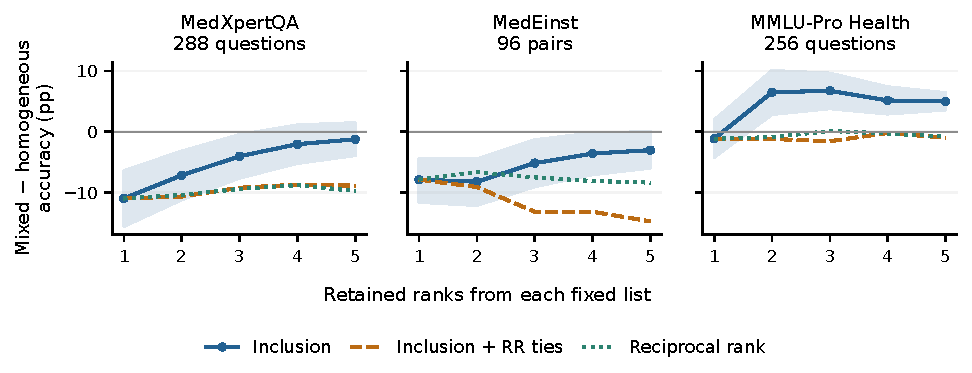
\includegraphics[width=\linewidth]{figures/REPRESENTATION_DEPTH.pdf}
\caption{Fixed-ballot depth replay, two banks per source. All curves coincide at depth one. At depth five, inclusion counts every answer equally; RR and the RR tie-breaker retain rank weights. Left/middle use the original four-model mixture; right uses $M_{44}$ versus $H_G$, as in the separate 720-case design. Bands are secondary paired 95\% intervals for inclusion; other curves are point estimates. $C$ compares paired endpoints, not marginal intervals. MedEinst uses refinements; both other sources use native keys.}
\label{fig:depth_supp}
\end{figure}


\begin{figure}[t]
\centering
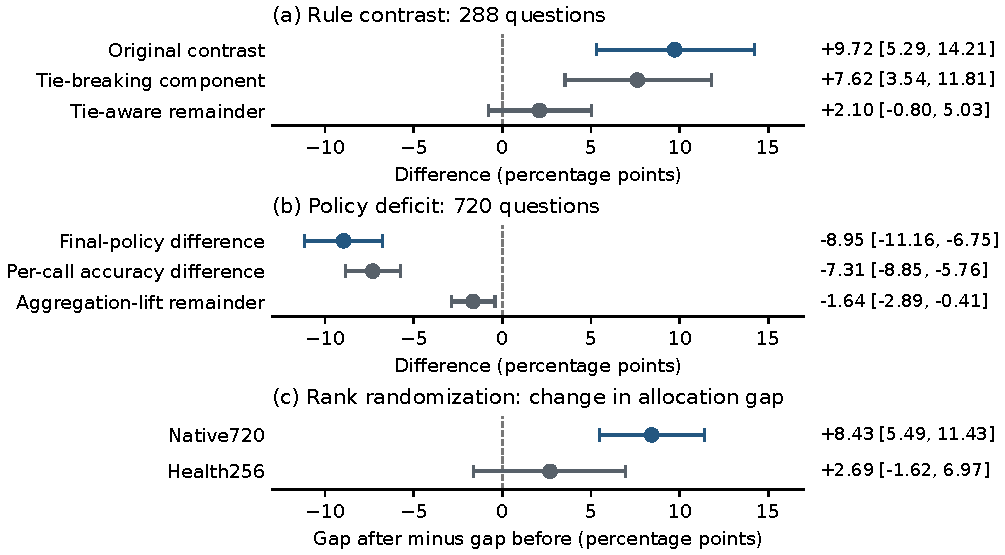
\includegraphics[width=\linewidth]{figures/PRIMARY_EXPLANATIONS.pdf}
\caption{Explanations and a rank intervention. (a,b) Rule and policy decompositions, with paired pointwise 95\% question-bootstrap intervals. Components add within each panel; their correlated intervals must not be added. (c) Paired change in the mixed-minus-Gemma first-choice gap after randomizing ranks, with intervals adjusted across eight endpoints. Both policies worsen; Health's change is unresolved. These exploratory analyses do not isolate a quality-independent lineage effect.}
\label{fig:explanations}
\end{figure}


The separate \path{eleven_review_replay.zip} contains stripped Native288/Native720/Health256 ballots, scored MedEinst rank pools, executable analyses, the exploratory specification, expected outputs and checksums. It contains no question text, credentials or new clinical labels. With Python and NumPy, run \texttt{python3 replay.py --data data --out outputs} and compare the three result files with \path{expected/}. The original eight-check archive remains unchanged. This replay does not regenerate hosted outputs or adjudicate the terminology map.

\subsection{Approval cutoff and tie handling on fixed responses}\label{app:cutoff}

This exploratory challenge asks whether the allocation comparison changes when approval counts only the first two answers rather than all five. It reuses the original Native288, Native720 and Health256 calls, keys, failures, allocations and two-bank averaging. No questions, model calls or clinical labels are added. Approval cutoff is the number of stored positions that receive a vote; it is not the number of answers requested during generation.

For cutoff $k\in\{2,5\}$, give each candidate in the first $k$ positions one vote per call. The uniform version averages all tied maximum-count candidates. The rank-tie version first maximizes approval count, then sums reciprocal ranks from \emph{all five positions} to resolve equal counts. Remaining ties are uniform. Only candidates receiving an approval vote are eligible. Thus the tie-breaker introduces additional preference information; it does not merely choose a deterministic candidate label. Empty allocations score zero. This is not a reproduction of the token-log-probability or additional-model tie procedure of \citet{wang2025ranked}.

Table~\ref{tab:cutoff_absolute} reports all absolute accuracies and tie rates. A tie rate is the proportion of question--bank decisions with multiple winners before the final uniform draw. In particular, Health's two-answer approval gain is not evidence that this policy beats the 68.82\% selected Gemma first-choice reference: its mixed accuracy is only 58.04\%. Adding rank information to break ties raises both allocations, and the mixed-minus-H difference becomes unresolved at $-1.17\ [-4.79,2.44]$ points (nominal paired 95\% interval).

\begin{table}[ht]
\centering\small
\caption{Fixed-response cutoff challenge. All values percent, except mixed-minus-H differences in points. Rank ties use the complete five-position RR score. First-choice and five-answer values reconcile exactly with the retained analyses. These are reused cases, not fresh confirmation.}
\label{tab:cutoff_absolute}
\begin{tabular}{llrrrrr}
\toprule
Source & Rule & H accuracy & M accuracy & M$-$H & H ties & M ties\\
\midrule
Native288 & First &29.86&18.91&$-10.95$&5.90&13.89\\
& Approval 2 &25.55&18.39&$-7.16$&40.45&16.84\\
& Approval 2, rank ties &28.82&18.92&$-9.90$&2.08&0.00\\
& Approval 5 &18.68&17.45&$-1.23$&94.27&66.84\\
& Approval 5, rank ties &29.51&20.66&$-8.85$&2.08&0.35\\
& RR &29.69&19.97&$-9.72$&2.08&0.52\\
\midrule
Native720 & First &35.21&26.26&$-8.95$&4.31&25.49\\
& Approval 2 &31.37&24.70&$-6.67$&37.71&29.24\\
& Approval 2, rank ties &34.93&24.76&$-10.17$&0.83&3.82\\
& Approval 5 &19.49&19.71&$0.22$&95.14&89.17\\
& Approval 5, rank ties &34.34&25.83&$-8.51$&1.04&3.82\\
& RR &34.65&24.86&$-9.79$&1.18&4.65\\
\midrule
Health256 & First &68.82&67.68&$-1.14$&2.54&20.70\\
& Approval 2 &51.56&58.04&$6.48$&60.94&39.06\\
& Approval 2, rank ties &69.43&68.26&$-1.17$&0.98&5.86\\
& Approval 5 &23.48&28.48&$5.00$&99.02&95.70\\
& Approval 5, rank ties &69.04&68.07&$-0.98$&0.98&5.27\\
& RR &69.04&68.26&$-0.78$&0.98&6.05\\
\bottomrule
\end{tabular}
\end{table}

Define $C_2$ as the cutoff-two allocation difference minus the first-choice allocation difference, $U_2$ as the same contrast with rank-resolved approval ties, and $T_2=C_2-U_2$. Resample whole questions 20,000 times within the original source/task strata, seed 20260923; banks remain together. The three $C_2$ contrasts form a three-endpoint family. The six $U_k$ contrasts (two cutoffs, three cohorts) and six $T_k$ contrasts each receive separate Bonferroni interval adjustment. Table~\ref{tab:cutoff_contrasts} shows the cutoff-two results. Native contrasts attenuate and become unresolved; Health retains a positive $C_2$, but not a resolved remainder after tie handling. An unresolved interval does not establish equivalence. Original primary estimates and their prespecified intervals are unchanged; these exploratory families do not retroactively adjust those tests.

\begin{table}[ht]
\centering\small
\caption{Cutoff-two rule contrasts and decomposition, points with family-adjusted 95\% paired intervals. $C_2=T_2+U_2$; correlated intervals must not be added.}
\label{tab:cutoff_contrasts}
\begin{tabular}{lrrr}
\toprule
Source & $C_2$ (three contrasts) & $T_2$ (six contrasts) & $U_2$ (six contrasts)\\
\midrule
Native288 & $3.79\ [-.41,7.93]$ & $2.73\ [-.52,6.00]$ & $1.06\ [-2.75,4.71]$\\
Native720 & $2.28\ [-.45,5.05]$ & $3.50\ [1.50,5.48]$ & $-1.22\ [-3.86,1.42]$\\
Health256 & $7.62\ [2.96,12.21]$ & $7.65\ [3.26,11.97]$ & $-.03\ [-3.42,3.37]$\\
\bottomrule
\end{tabular}
\end{table}

The separate \path{practical_cutoff_replay.zip} supplies stripped ballots, expected results, case vectors, checksums and a standalone program. Run \texttt{python3 replay.py --data data --out outputs}. Its 1,296 independent scalar checks include empty ballots, absent keys, reversed lists and partial lists; baseline means reconcile to $10^{-12}$. Compare both JSON outputs byte-for-byte with \path{expected/}. No network, GPU or model generation is needed.

\subsection{Published aggregation components and tie-choice robustness}\label{app:public_ties}

Could arbitrary uniform ties explain the native mixed-policy deficit? We test this rival without changing any generated answer. The BCV and MRRV classes released with \citet{wang2025ranked}, at commit \texttt{f5bb1c1}, accumulate Borda and reciprocal-rank scores, respectively, then return the first maximum encountered by \texttt{Counter.most\_common(1)}. We execute those classes on all three retained cohorts. Failed empty lists are represented by the source's invalid sentinel and excluded from vote accumulation; their questions remain, and an all-failure allocation scores zero. Native288 keeps its original four-model mixture; Native720 and Health keep their Gemma--Llama mixture.

This is an aggregation-component replay, not a reproduction of the published experiment. Our prompts, models, parser, ten-option questions and stored five-answer lists remain unchanged. The inspected code path has encounter-order tie handling, distinct from the paper-described confidence or extra-model resolution; we do not infer which path produced the authors' original results. Literal MRRV replay preserves floating-point additions. Reversing the eight input lists tests sensitivity to both encounter order and numerical summation, not a new generation order.

\begin{table}[t]
\centering\small
\caption{Published-component replay on existing answers. H/M accuracies are percentages; differences are percentage points. Scheduled-order differences have paired intervals adjusted across six source--rule contrasts. Reversed-order differences are descriptive sensitivity results, not selected policies.}
\label{tab:public_components}
\begin{tabular}{llrrrr}
\toprule
Source & Rule & H & M & M--H [adjusted 95\%] & Reversed\\
\midrule
Native288 & Borda &28.99&21.35&$-7.64\ [-13.83,-1.39]$&$-8.51$\\
& RR &29.69&19.97&$-9.72\ [-15.97,-3.47]$&$-9.72$\\
Native720 & Borda &35.07&25.97&$-9.10\ [-12.78,-5.69]$&$-11.11$\\
& RR &34.72&25.21&$-9.51\ [-13.17,-6.04]$&$-10.28$\\
Health & Borda &69.34&68.95&$-.39\ [-4.49,3.71]$&$-1.17$\\
& RR &68.95&68.55&$-.39\ [-4.69,3.91]$&$-.78$\\
\bottomrule
\end{tabular}
\end{table}

Both native cohorts retain a mixed deficit under both components; Health does not resolve one. Inference resamples questions 20,000 times within source/task, keeping two banks and all policies together, seed20260926. This exploratory six-contrast family does not alter the prespecified primary intervals. Reversing call order changes some estimates but not these observed directions (Table~\ref{tab:public_components}).

We also bound accuracy without specifying a tie-breaking algorithm. For each question--bank allocation, compute the exact set of maximum-score candidates, using rational reciprocal-rank scores. Its lower correctness is one only if gold is the sole maximizer; its upper correctness is one if gold is among the maximizers. Empty allocations have both endpoints zero. Average these endpoints over banks and questions. Subtract H's upper accuracy from M's lower for a lower bound on M--H; subtract H's lower from M's upper for an upper bound. This permits even gold-informed, allocation-specific tie choices: a deliberately generous outer envelope, not an attainable selector. It is not a confidence interval. A negative upper endpoint rules out reversal on these fixed outputs; an envelope containing zero does not demonstrate an operational reversal.

\begin{table}[t]
\centering\small
\caption{Fixed-output mixed-minus-H envelopes over arbitrary score-maximizing tie choices, in percentage points. These are gold-informed bounds, not sampling intervals. Inclusion bounds are deliberately broad because they permit adversarial resolution separately for each allocation.}
\label{tab:tie_envelopes}
\begin{tabular}{lrrrr}
\toprule
Source & First choice & Inclusion & RR & Borda\\
\midrule
Native288 &$[-14.93,-6.08]$&$[-55.38,34.90]$&$[-10.24,-9.20]$&$[-9.90,-6.42]$\\
Native720 &$[-16.04,-1.81]$&$[-61.67,54.24]$&$[-11.46,-8.12]$&$[-12.15,-7.92]$\\
Health &$[-9.38,7.03]$&$[-87.50,86.33]$&$[-3.12,1.56]$&$[-3.91,1.95]$\\
\bottomrule
\end{tabular}
\end{table}

Native720's first-choice upper bound is $-1.81$ points, but its nominal question-bootstrap interval is $[-3.89,.28]$: fixed-sample non-reversal does not establish population-level robustness for every tie policy. The RR/Borda upper-endpoint intervals are $[-10.83,-5.49]$ and $[-10.76,-5.21]$, respectively. Health envelopes cross zero. The results strengthen the native rank-rule deficit against a tie-choice explanation; they do not show that the positive inclusion interaction persists under realistic confidence-based aggregation or fresh prompts.

The \path{tie_policy_replay.zip} archive contains stripped inputs, the pinned source, independent checks and expected per-question outputs. Run \texttt{python3 replay.py --data data --source RankBasedSC.py --out outputs}. All 750 constructed checks and 20,224 actual-output comparisons against an independent literal implementation pass; original uniform-rule means reconcile to $10^{-12}$. No new model calls, labels, cases or costs are introduced. The analysis is post hoc and conditional on retained banks and keys.
